\subsection{Motivation}

The Machine Learning (ML) models (and in general the AI models) are expressed as minimiztion problems. In order to train ML we need to compute the \textit{best} parameters for the training data set.
The definition of \textit{best} is modelled by a minimizing (or maximizing) the objective function, usually called \textit{loss function}. 

The algorithms for minimizing or maximizing a function are called \textit{optimization algorithms}.

We can have unconstrained or constrained optimization, when constraints are imposed on the parameters to be determined.

Before introducing the optimization algorithms, we examine, as usual, the existence and uniqueness of the solution. In the following, we consider, as usual in optimization, minimization of functions. The maximization can be transformed to a suitable minimization problem.

The minimization of a function of several variables can be formulated as: given $f: \set{R}^n \rightarrow \set{R}$, called an \textit{objective function},
$$ \text{minimize } f(\vec{x}) \text{ in } \set{R}^n $$
This is called an \textit{unconstrained optimization problem}.

Typically, we want to determine the optimal values of several variables\\ $x_1, \hdots, x_n$ ruled by specific laws such as equality or inequality constraints. Moreover, we may require that these values lie within a subset $\Omega \subset \set{R}^n$. This kind of optimization problem is called \textit{constrained} and can be formulated as: given the objective function $f$,
$$ \text{minimize } f(\vec{x}) \text{ in } \Omega \subset \set{R}^n $$

In this chapter, we will address the following topics:
\begin{itemize}
    \item conditions for the existence (and uniqueness) of a solution
    \item numerical algorithms to solve these kinds of problems
\end{itemize}

\subsection{Preliminaries on multivariate functions}
\begin{definition}
    Let $f: \set{R}^n \rightarrow \set{R}$. We say that $f$ is \textit{differentiable} with respect to $x_i$ if the limit
    $$ \lim_{h \rightarrow 0}{\frac{f(x_1, \hdots, x_i+h, \hdots, x_n) - f(x_1, \hdots, x_n)}{h}} = \frac{\partial f}{\partial x_i}(\vec{x}) $$
    exists.
\end{definition}

\begin{definition}
    A function $f: \set{R}^n \rightarrow \set{R}$ is said differentiable at a point $\vec{x}_0 \in \set{R}^n$ iff all the partial derivatives of $f$ exists at $\vec{x}_0$.
\end{definition}


\begin{definition}
    Let $f: \set{R}^n \rightarrow \set{R}$ be a differentiable function. Then
    $$ \nabla{f}(\vec{x}) = \left( \frac{\partial f}{\partial x_1}(\vec{x}), \hdots, \frac{\partial f}{\partial x_n}(\vec{x}) \right) $$
    is called \textit{gradient} of $f$.
\end{definition}

\begin{definition}
    Let $f: \set{R}^n \rightarrow \set{R}$ be differentiable up to the second order. We call \textit{Hessian} the following matrix
    $$
        \mat{H}_f(\vec{x}) = \nabla^2{f}(\vec{x}) =
        \begin{bmatrix}
            \frac{\partial^2 f}{\partial x_1^2} & \frac{\partial^2 f}{\partial x_1 \partial x_2} & \cdots & \frac{\partial^2 f}{\partial x_1 \partial x_n}\\\\
            \frac{\partial^2 f}{\partial x_2 \partial x_1} & \frac{\partial^2 f}{\partial x_2^2} & \cdots & \frac{\partial^2 f}{\partial x_2 \partial x_n}\\\\
            \vdots & \vdots & \ddots & \vdots\\\\
            \frac{\partial^2 f}{\partial x_n \partial x_1} & \frac{\partial^2 f}{\partial x_n \partial x_2} & \cdots & \frac{\partial^2 f}{\partial x_n^2}
        \end{bmatrix}
    $$
\end{definition}


\begin{definition}
    Let $\vec{f}: \set{R}^n \rightarrow \set{R}^m$ be a function such that all its first-order partial derivatives exists. We call \textit{Jacobian} the following matrix
    $$
        \mat{J}_f(\vec{x}) = \frac{\partial\vec{f}}{\partial\vec{x}}(\vec{x}) =
        \begin{bmatrix}
            \nabla{f_1}(\vec{x})\\
            \nabla{f_2}(\vec{x})\\
            \vdots\\
            \nabla{f_m}(\vec{x})
        \end{bmatrix} =
        \begin{bmatrix}
            \frac{\partial f_1}{\partial x_1} & \frac{\partial f_1}{\partial x_2} & \hdots & \frac{\partial f_1}{\partial x_n}\\\\
            \frac{\partial f_2}{\partial x_1} & \frac{\partial f_2}{\partial x_2} & \hdots & \frac{\partial f_2}{\partial x_n}\\\\
            \vdots & \vdots & \ddots & \vdots\\\\
            \frac{\partial f_m}{\partial x_1} & \frac{\partial f_m}{\partial x_2} & \hdots & \frac{\partial f_m}{\partial x_n}
        \end{bmatrix}
    $$
\end{definition}

\begin{proposition}
    Let $\vec{f}: \set{R}^n \rightarrow \set{R}^m$ and $\vec{g}: \set{R}^m \rightarrow \set{R}^p$. The Jacobian matrix of the function $\vec{g} \circ \vec{f}: \set{R}^n \rightarrow \set{R}^p$ is given by
    $$ \mat{J}_{\vec{g} \circ \vec{f}}(\vec{x}) = \mat{J}_\vec{g}(\vec{f}(\vec{x})) \cdot \mat{J}_\vec{f}(\vec{x}) $$
\end{proposition}




\begin{definition}
    Let $f: \set{R}^n \rightarrow \set{R}$. $\vec{x}^* \in \set{R}^n$ is called a \textit{local minimum point} (resp. \textit{strict local minimum point}) of $f$ if there exists $\epsilon > 0$ such that
    $$ f(\vec{x}^*) \leq f(\vec{x})\ (\text{resp. } f(\vec{x}^*) < f(\vec{x})),\ \ \forall \norm{\vec{x} - \vec{x}^*} < \epsilon $$
\end{definition}

\begin{definition}
    Let $f: \set{R}^n \rightarrow \set{R}$. $\vec{x}^* \in \set{R}^n$ is called a \textit{global minimum point} (resp. \textit{strict global minimum point}) of $f$ if
    $$ f(\vec{x}^*) \leq f(\vec{x})\ (\text{resp. } f(\vec{x}^*) < f(\vec{x})),\ \ \forall \vec{x} \in \set{R}^n,\ \vec{x} \neq \vec{x}^* $$
\end{definition}

\begin{theorem} (First order optimality condition, also called Fermat's theorem for stationary points)
    Let $f: \set{A} \in \set{R}$, with $\set{U} \subseteq \set{R}^n$ open set. If $\vec{x}^* \in \set{U}$ is a local optimum point for $f$ and $f$ is differentiable in $\vec{x}^*$, then
    $$ \nabla{f}(\vec{x}^*) = 0 $$
\end{theorem}
Note that this is a necessary condition.

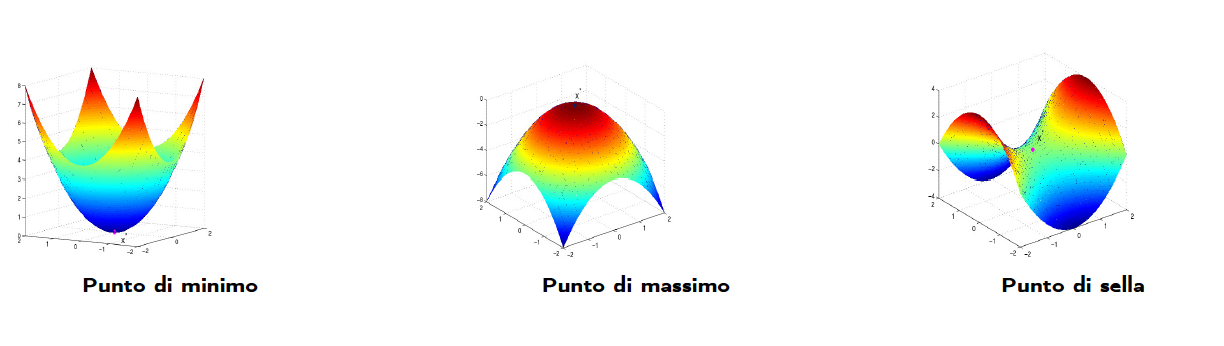
\includegraphics[width=0.9 \textwidth]{sections/images/opt1.png}


\begin{theorem} (Second order optimality condition)
    Let $f: \set{A} \in \set{R}$, with $\set{U} \subseteq \set{R}^n$ open set. If $\vec{x}^* \in \set{U}$ is a local minimum point for $f$ and $f$ is twice differentiable around $\vec{x}^*$, then
    $$ \nabla{f}(\vec{x}^*) = 0 \text{ and } \nabla^2{f}(\vec{x}^*) \text{ is positive semidefinite} $$
\end{theorem}
Note that this is a necessary condition.


\begin{theorem}
    If $f: \set{R}^n \rightarrow \set{R}$ is twice differentiable with continuity around $\vec{x}^* \in \set{R}^n$ and $\nabla{f}(\vec{x}^*) = 0$ and $\nabla^2{f}(\vec{x}^*)$ is positive definite, then $\vec{x}^*$ is a strict local minimum point.
\end{theorem}

\begin{definition}
    $\set{C} \subset \set{R}^n$ is a \textit{convex set} if $\forall\vec{x}, \vec{y} \in \set{C}$ and $\theta \in [0, 1]$ we have
    $$ \theta\vec{x} + (1 - \theta)\vec{y} \in \set{C} $$
\end{definition}

\begin{definition}
    Let $f: \set{D} \rightarrow \set{R}$, with $D \subset \set{R}^n$ convex set. Then $f$ is a \textit{convex function} if $\forall\vec{x}, \vec{y} \in \set{D}$, $\theta \in [0, 1]$ we have
    $$ f(\theta x + (1 - \theta)\vec{y}) \leq \theta f(\vec{x}) + (1 - \theta)f(\vec{y}) $$
\end{definition}

\begin{proposition}
    We have the following:
    \begin{itemize}
        \item If $f$ is twice differentiable in $\vec{x}$ and convex (resp. strictly convex), then $\nabla^2{f}(\vec{x})$ is positive semidefinite (resp. positive definite)
        \item If $f$ is a convex function then each point of local minimum is a point of global minimum
        \item If $f$ is strictly convex then there exists a unique point of global minimum
    \end{itemize}
\end{proposition}


\subsection{Iterative methods}
Iterative methods can be formulated as follows: given an initial vector $\vec{x}_0 \in \set{R}^n$, compute for $k \geq 0$ until convergence
$$ \vec{x}_{k+1} = g(\vec{x}_k) $$
where $g$ is an arbitrary function. We have that $\vec{x}_k \rightarrow \vec{x}^*$ for $k \rightarrow \infty$, where $\vec{x}^*$ is a stationary point (local minimum).

Since, for obvious reasons, we can't compute an infinite number of terms, we need to set a \textit{stopping criterion}. Some examples are:
\begin{itemize}
    \item \textit{absolute criterion} based on first order condition, $\norm{\nabla{f}(\vec{x}_k)} < \tau_A$, where $\tau_A$ is the chosen tolerance
    \item \textit{relative criterion}, $\frac{\norm{\nabla{f}(\vec{x}_k)}}{\norm{f}(\vec{x}_0)} < \tau_R$, where $\tau_R$ is the chosen tolerance
    \item \textit{absolute criterion} on succeeding values, $\norm{\vec{x}_{k+1} - \vec{x}_k} < \tau_{AP}$, where $\tau_{AP}$ is the tolerance
    \item \textit{relative criterion} on succeeding values, $\frac{\norm{\vec{x}_{k+1} - \vec{x}_k}}{\vec{x}_k} < \tau_{RP}$, where $\tau_{RP}$ is the tolerance
\end{itemize}

\textbf{Convergence speed}
In order to evaluate how fast the algorithm approximates the solution and to compare two or more different algorithms, we define the \textit{convergence speed}.

 Let $\vec P{x}_k$ be a sequence converging to $\vec{x}^*$.
\begin{itemize}
    \item \textbf{Q-linear} if it exists $r \in (0,1)$:
    $$\frac{\|\vec{x}_{k+1}-\vec{x}^*\|}{\|\vec{x}_{k}-\vec{x}^*\|} \leq r, \ \ \forall k > k^*$$
    Hence the distance from the solution decreases at each iteration of a constant factor.
    \item \textbf{Q-superlinear} if 
    $$\lim_k \frac{\|\vec{x}_{k+1}-\vec{x}^*\|}{\|\vec{x}_{k}-\vec{x}^*\|}=0$$
    \item \textbf{Q-quadratic}
    if $$\frac{\|\vec{x}_{k+1}-\vec{x}^*\|}{\|\vec{x}_{k}-\vec{x}^*\|^2} \leq M, \ \ \forall k > k^*$$
\end{itemize}

\textbf{Observation} We remark that the classical iterative optimization methods converge to a \textbf{stationary point} of the objective function. The stationary point not always is the global minimum of the function.


\subsection{Descent methods}
Descent methods are iterative methods that can be formulated as follows: given an initial vector $\vec{x}_0 \in \set{R}^n$, compute for $k \geq 0$ until convergence
$$ \vec{x}_{k+1} = \vec{x}_k + \alpha_k\vec{p}_k $$
where $\vec{p}_k$ is a suitably chosen descent direction and $\alpha_k$ is a positive parameter called \textit{stepsize} that measures the step along the direction $\vec{p}_k$. \\
This direction is called a \textit{descent direction} if   that there exists $\alpha_k > 0$ such that
$$ f(\vec{x}_k + \alpha_k\vec{p}_k) < f(\vec{x}_k) $$
We have that:
$$
    \begin{aligned}
        &\transp{\vec{p}}_k\nabla{f}(\vec{x}_k) < 0 &\text{ if } \nabla{f}(\vec{x}_k) \neq 0\\
        &\vec{p}_k = 0 &\text{ if } \nabla{f}(\vec{x}_k) = 0
    \end{aligned}
$$
provided that $f$ is continuously differentiable around $\vec{x}_k$.


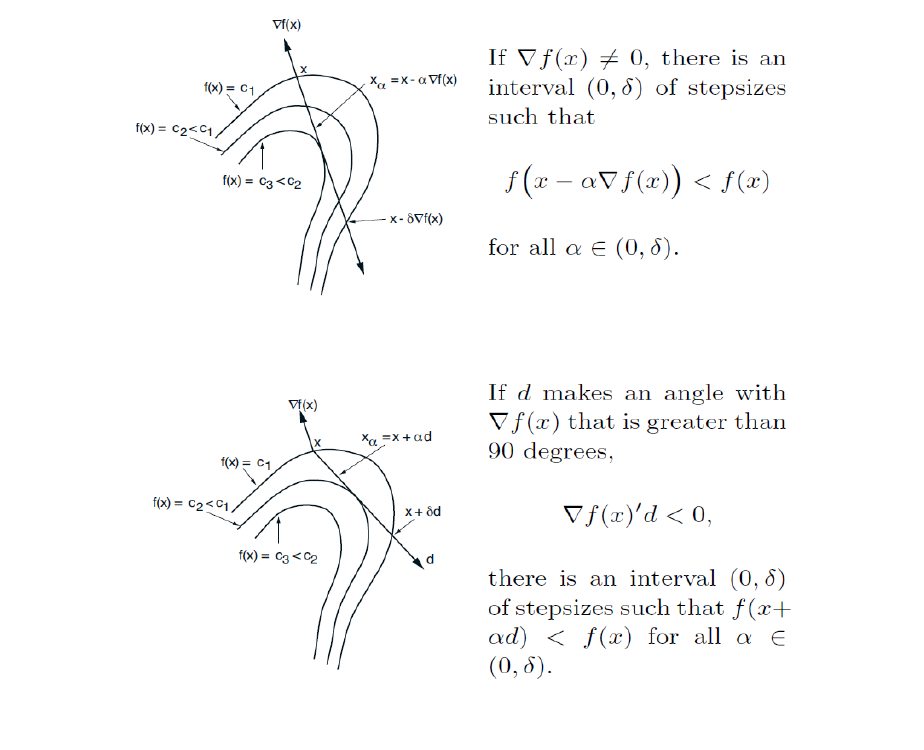
\includegraphics[width=0.9 \textwidth]{sections/images/opt3.png}

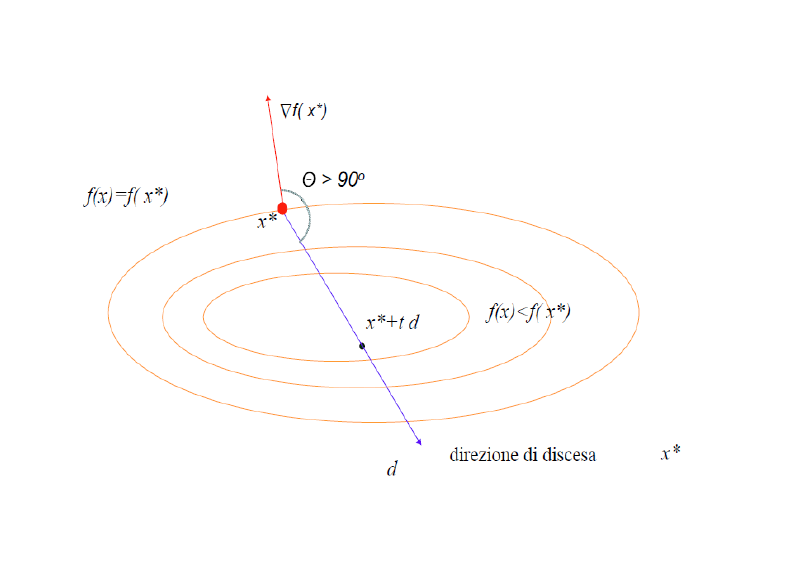
\includegraphics[width=0.7 \textwidth]{sections/images/opt4.png}

The choice of $\vec{p}_k$ corresponds to different methods.

\textbf{The choice of the step size}.

We observe that the choice of $\alpha_k$ so that:
$$f(\xx_{k+1})<f(\xx_k)$$ 
\textbf{doesn't guarantee the convergence of the method}.\\
Hence the choice of the step size is very important in a gradient descent method. If the step size is too small, the descent can be too slow. However, if the step size is too large, the method fails to converge. The step size is then usually chosen by a \textit{line search} algorithm implemented with a backtracking algorithm, where an iterative procedure decreases the value of the step size $\alpha$ until suitable conditions for the convergence of the method are satisfied. The method is called \textit{line search} since the new iterate $\xx_{k+1}$ is searched along the line $p_k$.

\begin{itemize}
    \item \textit{Exact line search}. $\alpha_k$ is chosen as the minimum of the function
    $$\Phi: R \longrightarrow R, \ \ \Phi(\alpha)=f(\xx_k+\alpha \vec{p}, \ \ \alpha \geq 0$$
    It is not the best way of choosing $\alpha_k$ in terms of converge speed of the algorithm.
    \item \textit{inexact line search}. $\alpha_k$ is chosen to belong to intervals where the algorithm convergence is guaranteed. The most common conditions which guarantees the convergence are the \textbf{Wolfe} conditions. 
    
    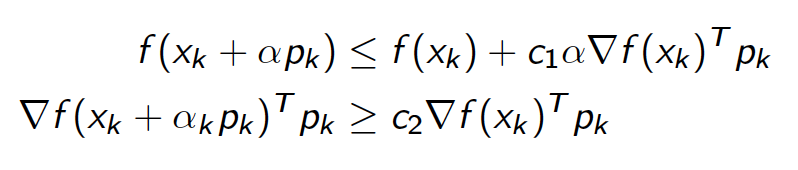
\includegraphics[width=0.7 \textwidth]{sections/images/opt5.png}
    
    with $0<c_1<c_2<1$.
    
    The first condition (Armijo condition) prevents ensures that $\alpha_k$ is not too large but it allows $\alpha_k$ to be too small. In this case the algorithm becomes very slow.\\
    The second condition (curvature condition) is a \textit{sufficient displacement} condition, preventing $\alpha_k$ from being too small.
    
    Since the curvature condition is computationally expensive, we can prove that the convergence is guaranteed if we apply a \textit{backtracking} algorithm that progressively reduces a starting values of $]\alpha$ usually set at one until the Armijo condition is satisfied. In the algorithm, a check condition ensures that $\alpha_k$ becomes not too small. In that case, the descent method is interrupted without convergence.
    
     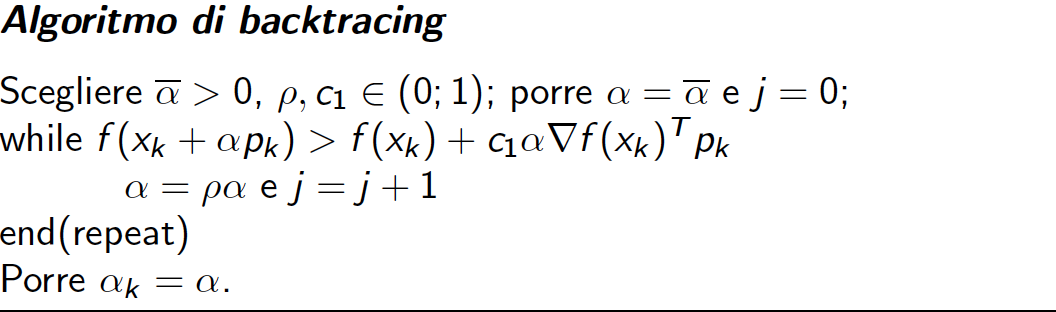
\includegraphics[width=0.7 \textwidth]{sections/images/opt6.png}
\end{itemize}



\subsubsection{Gradient descent method }

Gradient descent method is a first order optimization methods where the descent direction 
 is set as $\vec{p}_k = -\nabla{f}(\vec{x}_k)$.
 Thus
$$ \vec{x}_{k+1} = \vec{x}_k - \alpha\nabla{f}(\vec{x}_k) $$

A graphical representation can be seen in Figure \ref{fig:2}.

\begin{figure}
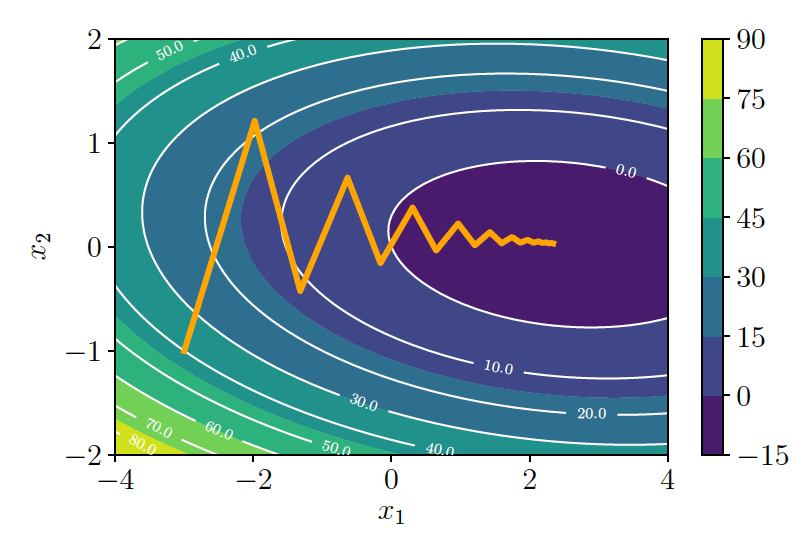
\includegraphics[width=0.7 \textwidth]{sections/images/opt2.png}
\caption{Gradient descent method on level curves of a quadratic function}
\label{fig:1}\end{figure}

The convergence speed of gradient methods is linear. In general, it can be quite slow.
 We can introduce a speeding technique called \textit{gradient descent with momentum}.
 It introduces a new term \textit{remembering} what happened in the previous iteration.
 The formula to update $\xx_k$ becomes:
 
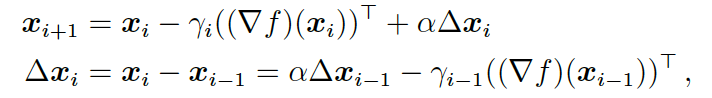
\includegraphics[width=0.7 \textwidth]{sections/images/opt7.png}

\subsubsection{Newton method}
It uses second order information of $f$, i.e. The Hessian of $f$.

The direction is set as
$$ \vec{p}_k = -\inv{H}_f(\vec{x}_k)\nabla{f}(\vec{x}_k) $$
provided that $\mat{H}_f$ is positive definite within a sufficiently large neighborhood of $\vec{x}^*$. At each iteration $\vec{p}_k$ is computed as a solution of the following linear system
$$ \mat{H}_f(\vec{x}_k)\vec{p}_k = \nabla{f}(\vec{x}_k) $$

\textbf{Convergence properties}
\begin{itemize}
    \item $\vec{p}_k$ is a decsent direction only if $\mat{H}_f$ is positive definite.
    \item The convergence properties are strictly realated to the Hessian matrix.
    \begin{proposition}
        If $f \in C^2(\Omega)$ and $\mat{H}_f$ is a Liptschiz function around $\xx^*$, i.e.
        $$|f(\xx) -f(\vec{y})| \leq K \|\xx-\vec{y} \|$$
        and $\mat{H}_f$ is positive definite then:
      if $\xx_0$ is near a stationary point $\xx^*$, then the sequence $\xx_k$ converges quadratically.
    \end{proposition}
    
\end{itemize}

\subsubsection{Possible changes in Newton methods}

\begin{itemize}
    \item 
 Approximate 
$\mat{H}_f(\vec{x}_k)$ with a positive definite matrix $\mat{B}_f(\vec{x}_k)$.
$$ \mat{H}_f(\vec{x}_k) \simeq \mat{B}(\vec{x}_k) $$ or by only using the first derivatives (\textit{Inexact Newton} methods).
\item Solve the linear system to compute the direction $p_k$ with iterative methods
\end{itemize}

\textbf{The role of the starting guess $\xx_0$.} We remark that the descent algorithms converge to a local minimum of the objective function. The value of the assigned vector $\xx_0$ starting the iterative procedure determines to which local minimum the algorithm converges. Obviously, we do not know a priori where the local (global) minima are located. If we have an estimate of the value we want to approximate, we can choose $\xx_0$ as near as possible to that value. In any case, we are not guaranteed which local minimum the algorithm converges to. In practice, we see that changing the starting guess, the result of algorithm can drastically change.

\subsection{Convex optimization}
Convex quadratic functions take the following form:
$$ q(\vec{x}) = \frac{1}{2}\transp{\vec{x}}\mat{Q}\vec{x} + \transp{\vec{c}}\vec{x}\ (+ \vec{w}) $$
with $\vec{x}, \vec{c} \in \set{R}^n$ and $\mat{Q} \in \set{R}^{n \times n}$ symmetric positive definite. A typical quadratic optimization problem is the least square problem
$$ \min{\norm{\mat{A}\vec{x} - \vec{b}}^2} $$
The objective is to minimize
$$
    \begin{aligned}
        \frac{1}{2}\norm{\mat{A}\vec{x} - \vec{b}}^2 &= \frac{1}{2}\transp{(\mat{A}\vec{x} - \vec{b})}(\mat{A}\vec{x} - \vec{b}) =\\
        &= \frac{1}{2}(\transp{\vec{x}}\transp{\mat{A}} - \transp{\vec{b}})(\mat{A}\vec{x} - \vec{b}) =\\
        &= \frac{1}{2}(\transp{\vec{x}}\transp{\mat{A}}\mat{A}\vec{x} - \transp{\vec{x}}\transp{\mat{A}}\vec{b} - \transp{\vec{b}}\mat{A}\vec{x} + \transp{\vec{b}}\vec{b}) =\\
        &= \frac{1}{2}\transp{\vec{x}}\transp{\mat{A}}\mat{A}\vec{x} - \transp{\vec{b}}\mat{A}\vec{x} + \frac{1}{2}\transp{\vec{b}}\vec{b}
    \end{aligned}
$$
which can be rewritten in quadratic form by setting $\mat{Q} = \transp{\mat{A}}\mat{A}$ and $\transp{\vec{c}} = -\transp{\vec{b}}\mat{A}$
We have
$$ \nabla{f}(\vec{x}) = \transp{\mat{A}}\mat{A}\vec{x} - \transp{\mat{A}}\vec{b}$$
and setting $\nabla{f}(\vec{x}) = 0$ we obtain the normal equations
$$ (\transp{\mat{A}}\mat{A})\vec{x} = \transp{\mat{A}}\vec{b} $$

A strictly convex function frequently encountered in applications is the quadratic function:
$$f(\xx)=\frac{1}{2} \xx^T Q \xx + \vec{b} ^T \xx$$
where $Q$ is a square matrix of size $n \times n$ symmetric and positive definite, $\vec{b} \in \mathbf{R}^n$.

In this particular case we have:
$$\nabla f(\xx)=Q \xx- \vec{b} \ \ \nabla^2 f(\xx)=A$$
Hence the unique minimizer of $f$ is the solution of the linear system representing the first order conditions $\nabla f(\xx)=0$:
$$Q \xx= \vec{b}$$

\textbf{Steepest descent method.} The \textit{steepest descent method} is the gradient method applied to a quadratic convex function with exact line search.

\begin{figure}
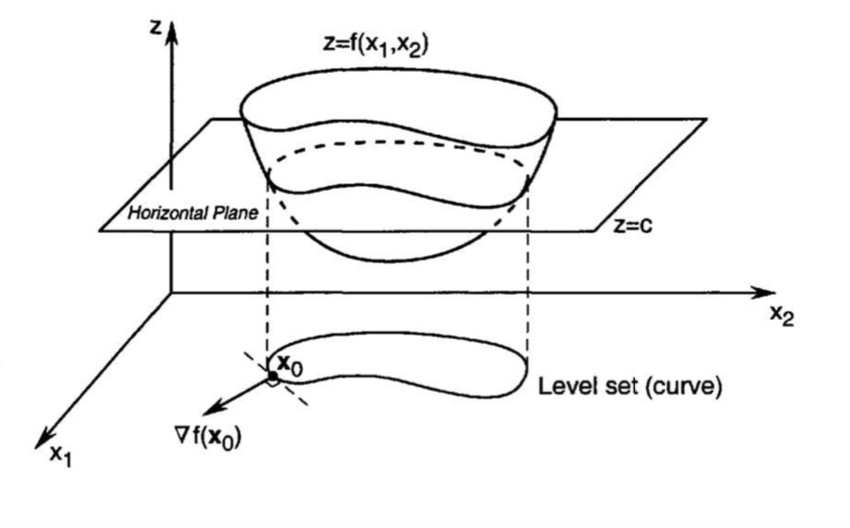
\includegraphics[width=0.7 \textwidth]{sections/images/opt8.png}
\caption{Descent direction in a gradient method}
\label{fig:2}\end{figure}

The step length $\alpha_k$ is computed as the global minimum of the univariate function of the variable $\alpha$ (in this case the function is convex):

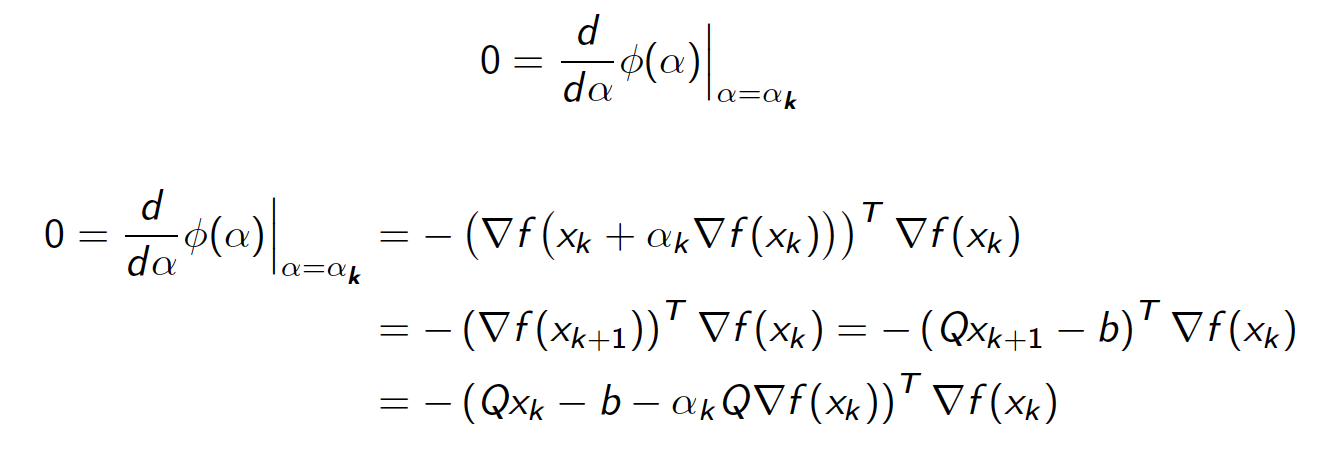
\includegraphics[width=0.9 \textwidth]{sections/images/opt12.png}

Hence:

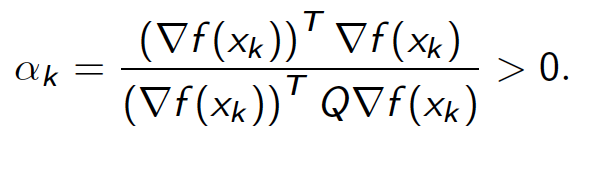
\includegraphics[width=0.5 \textwidth]{sections/images/opt13.png}

 The final algorithm can be written as:
 
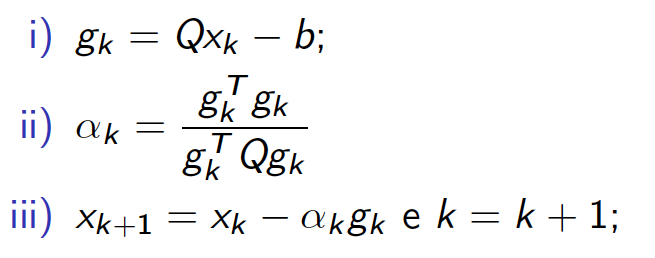
\includegraphics[width=0.6 \textwidth]{sections/images/opt14.png}


The gradient can be modified by considering Q-conjugate directions $\vec{p}_i$:
$$\vec{p}_i^T Q \vec{p}_j=0, \ \ if i \neq j$$

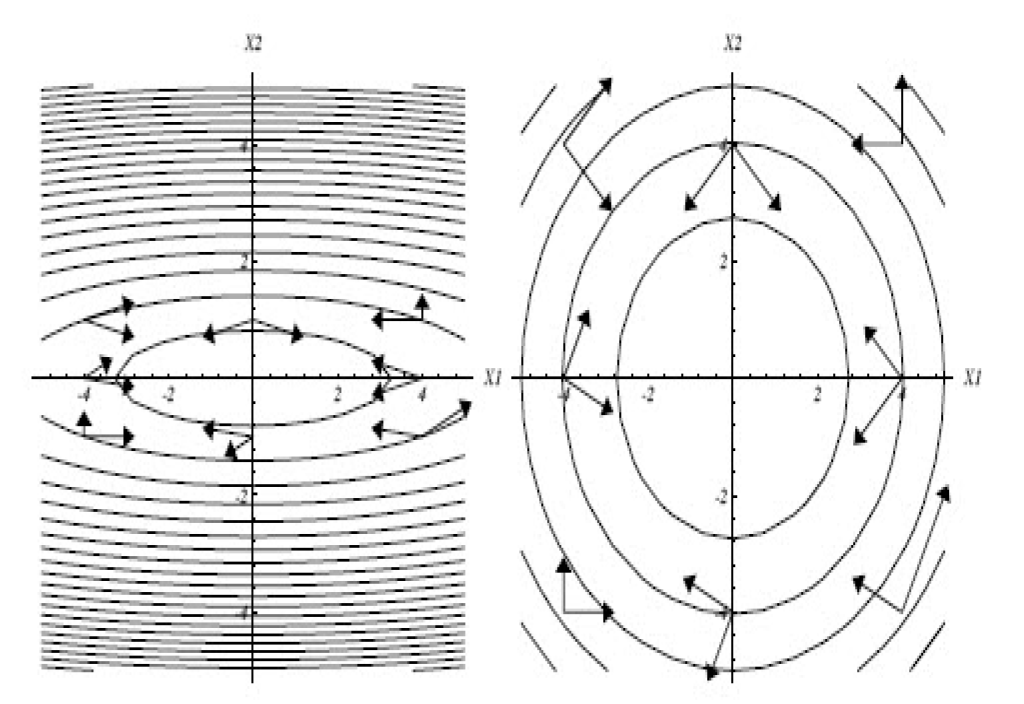
\includegraphics[width=0.6 \textwidth]{sections/images/opt9.png}
   
The \textit{Conjugate Gradient } (CG) algorithm is a very fast iterative algorithm for the minimization of a quadratic function (i.e. an iterative method for the solution of a linear system $Q\xx=\bb$ with $Q$ symmetric and positive definite).
It can be described by the following instructions:

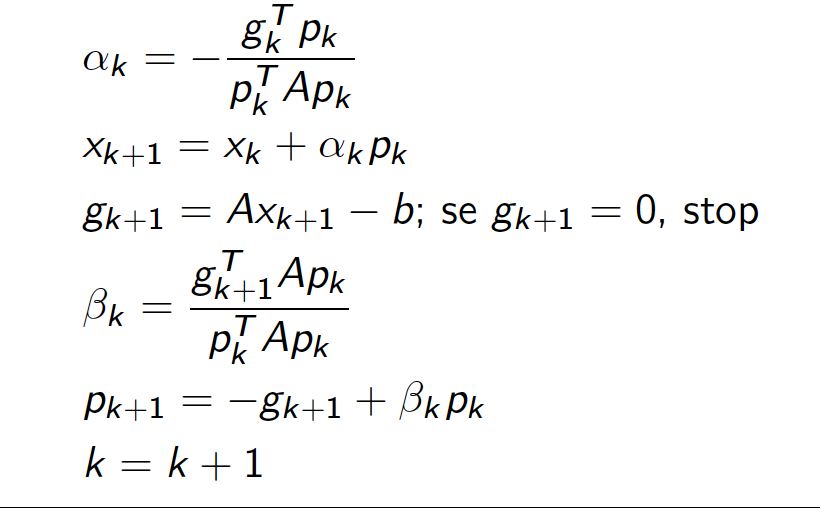
\includegraphics[width=0.6 \textwidth]{sections/images/opt10.png}

\begin{proposition}
If $A$ is symmetric and positive definite and it has at most $s$ distinct eigenvalues, then the CG method converges, in exact arithmetic, in at most $s$ iterations.
\end{proposition}

For any symmetric and positive definite matrix $Q$, we define the \textit{energy norm}:
$$\| \xx \|_Q=\sqrt{\xx^T Q \xx}$$ 
Concerning the convergence speed of Gradient Descent and Conjugate Gradient algorithms when applied to a quadratic function, we have the following results:
\begin{itemize}
\item For the steepest descent method it holds:
    $$ \| \xx_k - \xx^* \|_Q^2 \leq \left(\frac{K(Q)-1}{K(Q)+1}\right)^2 \| \xx_{k-1} - \xx^*\|_Q^2$$
    \item For the CG method it holds:
    $$ \| \xx_k - \xx^* \|_Q^2 \leq \left(\frac{K(Q)-1}{K(Q)+1}\right) \| \xx_{k-1} - \xx^*\|_Q^2 $$
\end{itemize}
where $k$ is the iteration number and $K(Q)$ is the condition number of $Q$.
Hence the CG method is quite faster then the Gradient descent method.

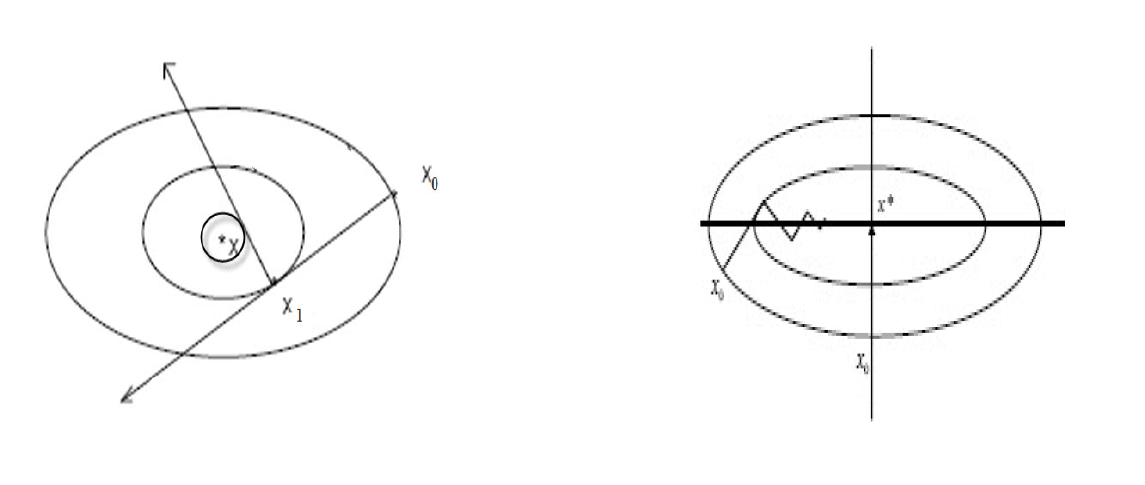
\includegraphics[width=0.6 \textwidth]{sections/images/opt15.png}

\subsection{Stochastic optimization}
The objective function in some ML problems is related to probabilistic events and it can take the following form
$$ G(\vec{x}) = \sum_{i = 1}^{n}{G_i(\vec{x})} $$
with $G: \set{R}^n \rightarrow \set{R}$. Each $G_i$ is the so called \textit{loss function} associated with the $i$-th observation in the dataset.
For example in a supervised classification problem we minimize the \textit{empirical risk function} $R_n:\mathbf{R}^d \longrightarrow \mathbf{R}$ defined as the sum of loss functions $l, \ i=1, \ldots n$ for all the examples $x_i$:
$$R_n(\vec{w})=\frac{1}{n} \sum_{i=1}^n l(h_(x_i,\vec{w}))$$
where the loss function $l$ is related to the probability distribution of the examples $x_i$.


In the case of standard (or \textit{batch}) gradient descent, the iteration is
$$
    \begin{aligned}
        \vec{x}_{k+1} &= \vec{x}_k - \alpha_k\nabla{G}(\vec{x}_k)\\
        &= \vec{x}_k - \alpha_k\sum_{i=1}^{n}{\nabla{G_i}(\vec{x}_k)}
    \end{aligned}
$$
When there are millions of examples, it is very expensive to compute the gradient $\nabla G(\xx)$.

In \textit{stochastic gradient descent} the true gradient $\nabla{G}(\vec{x}_k)$ is approximated at each iteration by the gradient at a single observation $\nabla{G_i}(\vec{x}_k)$, with $i = 1, \hdots, n$ randomly picked. The iteration step becomes
$$ \vec{x}_{k+1} = \vec{x}_k - \alpha_k\nabla{G_i}(\vec{x}_k) $$

A compromise between batch gradient descent and stochastic gradient descent is to compute the gradient against a set (called \textit{mini-batch}) of randomly picked observations. This method is therefore called \textit{mini-batch stochastic gradient descent}. The iteration step becomes
$$ \vec{x}_{k+1} = \vec{x}_k - \alpha_k\sum_{i \in M}{\nabla{G_i}(\vec{x}_k)},\ \ \ M \subset \{1, \hdots, n\} $$
The selection of the set $M$ can be performed in different random ways and it can also depend on the iterate $\xx_k$.

The step size $\alpha_k$ can be fixed or dynamically computed with a line search procedure. Both the choices are interesting in ML.

Each iteration is now very cheap and $\xx_1, \ldots \xx_k $ is a stochastic process, whose behaviour is determined by the random sequence $i_1, \ldots i_k$ of the indices of the computed component of the gradient at each iteration (in the case of a single component or depending on the random sequence of the mini-batches).
Even if the direction $-\nabla G_{i_k}(\xx_k)$ might NOT be a descent direction from $\xx_k$, but it is a descent direction \textit{in expectation}. This is proved to converge \textit{in expectation} to a local minumum of $G$.

Stochastic gradient descent is less computationally demanding with respect to batch gradient descent, but its convergence speed is lower. The convergence of stochastic gradient descent has been analyzed using the theories behind convex minimization and stochastic approximation.
Since in ML we do not need a very precise localization of the minimum of the function, stochastic (or mini-batch) gradient represents a very good compromise between precision and computational cost and it is widely used in practice, such as in neural network training algorithms.

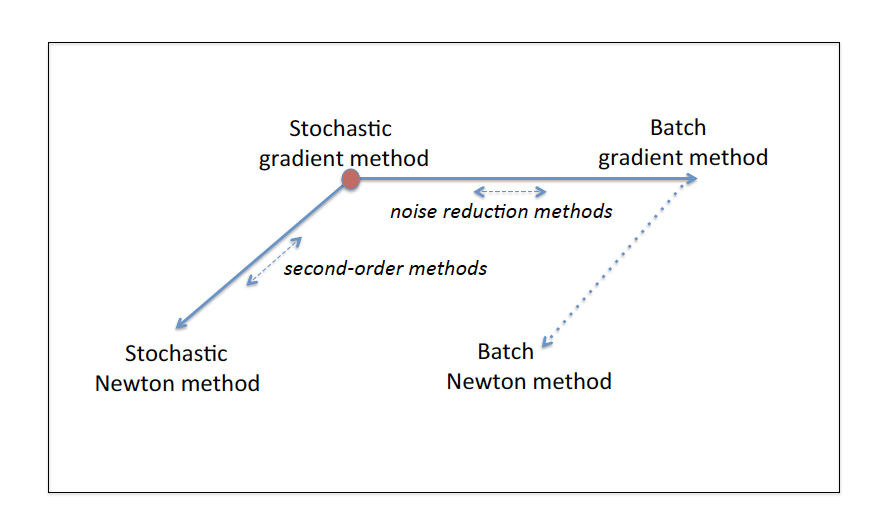
\includegraphics[width=0.6 \textwidth]{sections/images/opt11.png}

In a similar way, other optimization algorithms, such as Newton-like methods , can be implemented with a stochastic (or mini-batch) gradient computation.
More details can be found in \textit{Optimization for large scale machine learning, Siam Review, vol. 60, n.2, pag. 223-311, 2018}, where some convergence results are presented in the case of strictly convex functions.

\subsection{Non-linear least squares problem}
In non-linear least squares problems we have residuals defined as $\vec{r}: \set{R}^n \rightarrow \set{R}^m$, where $n$ is the dimension of the space of the data and $m$ is the dimension of the space of the unknowns. Each $r_i(\vec{x})$ is a non-linear function and the minimization of the residuals can be written as
$$ \min{\norm{\vec{r}(\vec{x})}^2} = \min{\sum_{i = 1}^{m}{r_i^2(\vec{x})}} $$
We can write the gradient of $f: \set{R}^m \rightarrow \set{R}$, $f = \frac{1}{2}\sum_{i = 1}^{m}{r_i^2(\vec{x})}$ as
$$ \nabla{f}(\vec{x}) = \sum_{i = 1}^{m}{r_i(\vec{x})\nabla{r_i}(\vec{x})} = \transp{\mat{J}}_r(\vec{x}) \cdot \vec{r}(\vec{x}) $$
and the hessian of $f$ as
$$
    \begin{aligned}
        \mat{H}_f(\vec{x}) &= \sum_{i = 1}^{m}{\left(\nabla{r_i}(\vec{x}) \cdot \nabla^T{r_i}(\vec{x}) +\nabla{r_i}(\vec{x}) \cdot \transp{\mat{H}}_{r_i}(\vec{x})\right)} =\\
        &= \transp{\mat{J}}_r(\vec{x}) \cdot \mat{J}_r(\vec{x}) + \sum_{i = 1}^{m}{\nabla{r_i}(\vec{x}) \cdot \transp{\mat{H}}_{r_i}(\vec{x})}
    \end{aligned}
$$

These formulas can be very expensive to compute. The methods used to solve these problems are:
\begin{itemize}
    \item \textit{gradient methods}
    \item \textit{Newton-like methods}
    \item \textit{Gauss-Newton method}, where $\vec{p}_k$ is computed as
    $$ (\transp{\mat{J}}_r \cdot \mat{J}_r)(\vec{x}_k) \cdot \vec{p}_k = -\transp{\mat{J}}_r(\vec{x}_k) \cdot \vec{r}(\vec{x}_k) $$
    \item \textit{Levenberg-Marquardt method}, adds regularization because $(\transp{\mat{J}}_r \cdot \mat{J}_r)$ can be ill-conditioned. $\vec{p}_k$ is computed as
    $$ (\transp{\mat{J}}_r(\vec{x}_k) \cdot \mat{J}_r(\vec{x}_k) + \lambda\mat{I}) \cdot \vec{p}_k = -\transp{\mat{J}}_r(\vec{x}_k) \cdot \vec{r}(\vec{x}_k) $$
\end{itemize}

\subsection{Constrained optimization. Lagrange multipliers}

We consider now the problem
\begin{eqnarray}
& min_x G(\xx) \\
& s.t. \ h_i(\xx) \leq 0 \ i=1, \ldots m
\label{eq:1}
\end{eqnarray}

A possible way of solving \eqref{eq:1} is to introduce the \textit{Lagrange multipliers} $\lambda_i \geq 0, \ i=1, \ldots m.$ The \textit{Lagrangian} function associated to problem \eqref{eq:1}. is:
$$L(\xx, \vec{\lambda})=G(\xx)+\sum_{i=1}^m \lambda_i h_i(\xx)$$

Many numerical methods use also the concept of duality. The minimization in a set of variables, say $\xx$ is moved in the minimization in another set of variables, say $\vec{\lambda}$. Given a minimization problem, there is not a unique way of getting duality. We consider now the so called \textit{Lagrangian duality}.

\begin{definition}
To the \textit{primal problem} \eqref{eq:1} with primal variables $\xx$, we associate the \textit{Lagrangian dual problem} in the form:
\begin{eqnarray*}
max_{\vec{\lambda}\in R^m} D(\vec{\lambda}) \\
s.t. \ \vec{\lambda} \geq 0
\end{eqnarray*}
where $D(\vec{\lambda})=min_{\xx \in R^n} L(\xx, \vec{\lambda})$ and $\vec{\lambda}$ are the \textit{dual variables}.
\end{definition}

The first one is the \textit{minimax problem}. If the solution of $min_{\xx \in R^n} L(\xx, \vec{\lambda})$ can be easily performed, then all the problem can be effortlessly computed. In fact, the maximization problem of $D(\vec{\lambda})$ is a concave problem, whose maximum is quite simple to find, even if $G$ and $h_i$ are not convex.

A particular case is the case when the functions $G$ and $h_i$ are linear. In this case we obtain the \textit{linear programming problem}

% \subsection{Regularization}
% \textit{Regularization} techniques can be used to slightly change ill-conditioned matrices. The simplest method is to add a diagonal matrix multiplied by a \textit{regularization parameter}, $\lambda\mat{I}$. Regularization also attempts to impose Occam's razor on the solution, meaning that it helps generate a simpler solution which is less affected by noise. For example, in Bayesian statistics we can impose certain prior distributions (regularization term) on model parameters
% $$ \hat{\theta}_{MAP} = -\argmin_{\theta}{\sum_{i = 1}^{n}{\log{f_X(x_i \mid \theta)}}} + \lambda\log{p(\theta)} $$

